\chapter{Generative Learning Algorithms}
So far, we’ve mainly been talking about learning algorithms that model $p(y | x; \theta)$, 
the conditional distribution of $y$ given $x$; for instance, logistic regression modeled $p(y | x; \theta)$ as
$h_{\theta}(x) = g(\transpose{\theta}x)$ where $g$ is the sigmoid function.

In these notes, we’ll talk about a different type of learning algorithm: consider a classification problem
in which we want to learn to distinguish between elephants ($y = 1$) and dogs ($y = 0$), based on some features
of an animal and given a training set, an algorithm like logistic regression or the perceptron algorithm
tries to find a straight line, that is, a decision boundary, that separates the elephants and dogs.

Then, to classify a new animal as either an elephant or a dog, it checks on which side of the decision boundary
it falls, and makes its prediction accordingly but now we introduce a different approach.

First, looking at elephants, we can build a model of what elephants look like, then, looking at dogs,
we can build a separate model of what dogs look like, so finally, to classify a new animal,
we can match the new animal against the elephant model, and match it against the dog model, 
to see whether the new animal looks more like the elephants or more like the dogs we had seen in the training set.

Algorithms that try to learn $p(y | x)$ directly (such as logistic regression), or algorithms that try to learn 
mappings directly from the space of inputs $X$ to the labels $\{0, 1\}$
are called \emph{discriminative learning algorithms}.

Here, we’ll talk about algorithms that instead try to model $p(x; y)$ and $p(y)$ and these algorithms
are called \emph{generative learning algorithms}; for instance, if $y$ indicates whether an example is
a dog $(0)$ or an elephant $(1)$, then $p(x | y = 0)$ models the distribution of dogs’ features, and 
$p(x | y = 1)$ models the distribution of elephants’ features.

After modeling $p(y)$, called the \emph{class priors} and $p(x; y)$, our algorithm can then use Bayes rule
to derive the posterior distribution on $y$ given $x$
\[ p(y | x) = \frac{p(x | y)p(y)}{p(x)} \]
where the denominator is given by 
\[ p(x) = p(x | y = 1)p(y = 1) + p(x | y = 0)p(y = 0) \] 
and thus can also be expressed in terms of the quantities $p(x |y)$ and $p(y)$ that we’ve learned.

Actually, if were calculating $p(y | x)$ in order to make a prediction, then we don’t actually need to 
calculate the denominator, since 
\begin{align*}
 arg \, max_y p(y | x) & = arg \, max_y \, \frac{p(x; y)p(y)}{p(x)} \\
                      & = arg \, max_y \, p(x;y)p(y) \\
\end{align*}

\section{Gaussian discriminant analysis}
The first generative learning algorithm that we’ll look at is \emph{Gaussian discriminant analysis(GDA)} and 
in this model, we’ll assume that $p(x | y)$ is distributed according to a multivariate normal distribution.

The \emph{multivariate normal distribution} in $n$-dimensions, also called the multivariate Gaussian distribution,
is parameterized by a mean vector $\mu \in \R ^ n$ and a covariance matrix $\Sigma \in \R ^ {n \times n}$,
where $\Sigma \geq 0$ is symmetric and positive semidefinite.

Also written as $N(\mu, \Sigma)$ its density is given by
\[ P(x; \mu, \Sigma) = \frac{1}{(2\pi)^{n/2} |\Sigma|^{1/2}} exp(- \frac{1}{2}(x - \mu)^T \Sigma ^{-1} (x -\mu)) \]
In the equation above, $|\Sigma|$ denotes the determinant of the matrix $\Sigma$ and for a random variable
$X$ distributed as $N(\mu, \Sigma)$, the mean is (unsurprisingly) given by $\mu$
\[ E[X] = \int _x x  p(x; \mu, \Sigma) dx= \mu \]
The covariance of a vector-valued random variable $Z$ is defined as 
\[ Cov(Z) = E[(Z - E[Z])(Z - E[Z])^T] \]
This generalizes the notion of the variance of a real-valued random variable 
and the covariance can also be defined as 
\[ Cov(Z) = E[ZZ^T] - (E[Z])(E[Z])^T \]
If $X \sim N(\mu, \Sigma)$ then $Cov(X) =  \Sigma$ 
%and also in figure \ref{img:multivariate} and \ref{img:multiCov}
%is possible to see some examples of what the density of a Gaussian distribution looks like.

\subsection{The Gaussian Discriminant Analysis model}
When we have a classification problem in which the input features $x$ are continuous valued random variables,
we can then use the Gaussian Discriminant Analysis(GDA) model, which models $p(x; y)$ using a
multivariate normal distribution, as we can see now:
\begin{align*}
    y & \sim Bernoulli(\phi) \\
    x|y = 0 & \sim  N(\mu_0, \Sigma) \\
    x|y = 1 & \sim  N(\mu_1, \Sigma) \\
\end{align*}
Writing out the distributions, we obtain that 
\begin{align*}
    p(y) & = \phi^y (1 - \phi)^{1-y} \\
    p(x| y = 0) & = \frac{1}{(2\pi)^{n/2} |\Sigma|^{1/2}} exp(-\frac{1}{2}(x - \mu_0)^T \Sigma^{-1} (x - \mu_0)) \\
    p(x| y = 1) & = \frac{1}{(2\pi)^{n/2} |\Sigma|^{1/2}} exp(-\frac{1}{2}(x - \mu_1)^T \Sigma^{-1} (x - \mu_1)) \\    
\end{align*}
Here, the parameters of our model are $\phi, \Sigma, \mu_0$ and $\mu_1$ (note that while there’re 
two different mean vectors $\mu_0$ and $\mu_1$, this model is usually applied using only 
one covariance matrix $\Sigma$) and the log-likelihood of the data is given by 
\begin{align*}
    l(\phi, \mu_0, \mu_1, \Sigma) & = \log \sum _{i=1}^m p(x^{(i)}, y^{(i)}; \phi, \mu_0, \mu_1, \Sigma) \\
                                  & = \log \sum _{i=1}^m p(x^{(i)} | y^{(i)}; \mu_0, \mu_1, \Sigma) p(y^{(i)}; \phi) 
\end{align*}
By maximizing $l$ with respect to the parameters, we find the maximum likelihood estimate of the parameters to be
\begin{align*}
    \phi & = \frac{1}{m} \sum _{i=1} ^ m 1\{y^{(i)} = 1 \} \\
    \mu_0 & = \frac{\sum _{i=1} ^ m 1\{y^{(i)} = 0\}x(i)}{\sum _{i=1} ^ m 1\{y^{(i)} = 0\}} \\
    \mu_1 & = \frac{\sum _{i=1} ^ m 1\{y^{(i)} = 1\}x(i)}{\sum _{i=1} ^ m 1\{y^{(i)} = 1\}}\\    
    \Sigma & = \frac{1}{m} \sum _{i=1}^m \transpose{(x^{(i)} - \mu _{y^(i)}) (x^{(i)} - \mu _{y^{(i)}})}
\end{align*}
Pictorially, what the algorithm is doing can be seen in figure \ref{img:gdaExample}.

\begin{figure}
    \caption{GDA representation example}
    \label{img:gdaExample}
    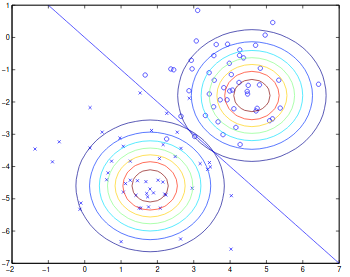
\includegraphics[width=\textwidth]{images/gda}
\end{figure}

\subsection{Discussion: GDA and logistic regression}

The GDA model has an interesting relationship to logistic regression, in fact if we view the quantity 
\[ p(y = 1 | x; \phi, \mu_0, \mu_1, \Sigma) \]
as a function of $x$, we’ll find that it can be expressed in the form
\[ p(y = 1 | x; \phi, \Sigma, \mu_0, \mu_1) = \frac{1}{1 + exp(-\transpose{\theta}x)} \]
where $\theta$ is some appropriate function of $\phi, \Sigma, \mu_0, \mu_1$.

This is exactly the form that logistic regression, a discriminative algorithm, used to model 
$p(y = 1 | x)$ and GDA and logistic regression will, in general, give different decision boundaries
when trained on the same dataset.\newline
We just argued that if $p(x | y)$ is multivariate gaussian(with shared $\Sigma$), then $p(y | x)$
necessarily follows a logistic function and the converse, however, is not true, so $p(y | x)$
being a logistic function does not imply $p(x | y)$ is multivariate gaussian.

This shows that GDA makes stronger modeling assumptions about the data than does logistic regression and 
it turns out that when these modeling assumptions are correct, then GDA will find better fits to the data, 
so it is a better model.

Specifically, when $p(x | y)$ is indeed gaussian (with shared $\Sigma$), then GDA is asymptotically efficient
and informally, this means that in the limit of very large training sets, there is no algorithm that
is strictly better than GDA, in terms of how accurately they estimate $p(y |x)$.

In particular, it can be shown that in this setting, GDA will be a better algorithm than logistic regression
and more generally, even for small training set sizes, we would generally expect GDA to better.\newline
In contrast, by making significantly weaker assumptions, logistic regression is also more robust 
and less sensitive to incorrect modeling assumptions and there are many different sets of assumptions that
would lead to $p(y |x)$ taking the form of a logistic function; for example, if $x | y = 0 \sim Poisson(\lambda_0)$,
and $x | y = 1 \sim Poisson(\lambda_1)$, then $p(y | x)$ will be logistic.

Logistic regression will also work well on Poisson data like this, but if we were to use GDA on such data,
and fit Gaussian distributions to such non-Gaussian data, then the results will be less predictable,
and GDA may (or may not) do well.

Specifically, when the data is indeed non-Gaussian, then in the limit of large datasets, logistic regression will
almost always do better than GDA and for this reason, in practice logistic regression is used more often than GDA.

\section{Naive Bayes}
In GDA, the feature vectors $x$ were continuous, real valued vectors and let’s now talk about a 
different learning algorithm in which the $x_j$’s are discrete-valued.

For our motivating example, consider building an email spam filter using machine learning and here,
we wish to classify messages according to whether they are unsolicited commercial(spam) email, or non-spam email.

After learning to do this, we can then have our mail reader automatically filter out the spam messages and
perhaps place them in a separate mail folder: classifying emails is one example of a broader set of problems
called \emph{text classification}.

Let’s say we have a training set (a set of emails labeled as spam or non-spam) and we’ll begin our construction
of our spam filter by specifying the features $x_j$ used to represent an email.

We will represent an email via a feature vector whose length is equal to the number of words in the dictionary and 
specifically, if an email contains the $j$-th word of the dictionary, then we will set $x_j = 1$ otherwise,
we let $x_j = 0$ so for instance, the vector 
\[ x = \begin{bmatrix}
    1 \\
    0 \\
    \vdots \\
    1 \\
    \vdots \\
    0 \\
       \end{bmatrix} \]
is used to represent an email that contains the words "a" and "buy" but not "aardvark", "aardwolf" 
or "zygmurgy.".

The set of words encoded into the feature vector is called the \emph{vocabulary}, so the dimension of
$x$ is equal to the size of the vocabulary and having chosen our feature vector, 
we now want to build a generative model, so we have to model $p(x | y)$.

If we have a vocabulary of $50000$ words, then $x \in \{0, 1\}^{50000}$ and if we were to model $x$
explicitly with a multinomial distribution over the $2^{50000}$ possible outcomes, then we’d end up 
with a $(2^{50000} - 1)$-dimensional parameter vector so this is clearly too many parameters.

To model $p(x |y)$, we will therefore make a very strong assumption, so we will assume that the $x_i$’s
are conditionally independent given $y$ and this assumption is called the Naive Bayes (NB) assumption,
and the resulting algorithm is called the \emph{Naive Bayes classifier}.

We now have 
\begin{align*}
    p(x_1, \dots, x_{50000} | y) & = p(x_1 | y)p(x_2 | y, x_1)p(x_3 | y, x_1, x_2) \dots 
                                     p(x_{50000} | y, x_1, \dots, x_{49999}) \\
                                 & = p(x_1 | y)p(x_2| y)p(x_3 | y)\dots p(x_{50000} | y) \\
                                 & = \prod _{i=1}^n p(x_i | y) 
\end{align*}
The first equality simply follows from the usual properties of probabilities, the second equality used
the NB assumption and we note that even though the Naive Bayes assumption is an extremely strong assumptions,
the resulting algorithm works well on many problems.

Our model is parameterized by $\phi_{j | y = 1} = p(x_j = 1 | y = 1)$, $phi_{j | y = 0} = p(x_j = 1 | y = 0)$,
and $\phi_y = p(y = 1)$ and as usual, given a training set $\{(x^{(i)}, y^{(i)}) \forall i =1, \dots, m \}$,
we can write down the joint likelihood of the data as
\[ L(\phi_y, \phi_{j | y = 0}, \phi_{j | y = 1}) = \prod _{i = 1}^ m p(x^{(i)}, y^{(i)}) \]
Maximizing this with respect to $\phi_y, \phi_{j | y = 0}$ and $\phi_{j | y = 1}$ 
gives the maximum likelihood estimates
\begin{align*}
    \phi_{j | y = 1} & = \frac{\sum _{i=1} ^ m 1\{x_j^{(i)} = 1 \land y^{(i)} = 1\}}{\sum _{i=1}^m 1\{y^{(i)} = 1\}} \\
    \phi_{j | y = 0} & = \frac{\sum _{i=1} ^ m 1\{x_j^{(i)} = 1 \land y^{(i)} = 0\}}{\sum _{i=1}^m 1\{y^{(i)} = 0\}} \\
    \phi_j           &= \frac{\sum _{i=1} ^ m 1\{y^{(i)} = 1\}}{m}
\end{align*}
Having fit all these parameters, to make a prediction on a new example with features $x$,
we then simply calculate 
\begin{align*}
    p(y = 1 | x) & = \frac{p(x | y = 1)p(y = 1)}{p(x)} \\
                 & = \frac{\left(\sum _{j = 1}^n p(x_j | y = 1) \right) p(y = 1)}
                          {\left(\sum _{j = 1}^n p(x_j | y = 1) \right) p(y = 1) +
                           \left(\sum _{j = 1}^n p(x_j | y = 1) \right) p(y = 0)} 
\end{align*}
and pick whichever class has the higher posterior probability.

Lastly, we note that while we have developed the Naive Bayes algorithm mainly for the case of problems
where the features $x_j$ are binary valued, the generalization to where $x_j$ can take values in 
$\{1, 2, \dots, k_j\}$ is straightforward, so we would simply model $p(x_j | y)$ as multinomial rather
than as Bernoulli.

Indeed, even if some original input attribute were continuous valued, it is quite common to discretize it,
that is, turn it into a small set of discrete values, and apply Naive Bayes.

\section{Laplace smoothing}
The Naive Bayes algorithm as we have described it will work fairly well for many problems,
but there is a simple change that makes it work much better, especially for text classification.

Let’s briefly discuss a problem with the algorithm in its current form, and then talk about how we can fix it
so we consider spam/email classification, and let’s suppose that, after completing the ML course,
you decide to submit the work you did to the NIPS conference for publication (NIPS is one of the top 
machine learning conferences, and the deadline for submitting a paper is typically in late June or early July).

Because you end up discussing the conference in your emails, you also start getting messages 
with the word “nips” in it, but this is your first NIPS paper, and until this time, you had not previously
seen any emails containing the word “nips”; in particular “nips” did not ever appear in your training set
of spam/non-spam emails.

Assuming that “nips” was the $35000$-th word in the dictionary, your Naive Bayes spam filter therefore
had picked its maximum likelihood estimates of the parameters $\phi_{35000| y}$ to be
\begin{align*}
    \phi_{35000 | y = 1} & = \frac{\sum _{i=1}^m 1\{x_{35000}^{(i)} = 1 \land y^{(i)} = 1\}}
                                  {\sum _{i=1}^m 1\{y^{(i)} = 1\}} \\
    \phi_{35000 | y = 0} & = \frac{\sum _{i=1}^m 1\{x_{35000}^{(i)} = 1 \land y^{(i)} = 0\}}
                                  {\sum _{i=1}^m 1\{y^{(i)} = 0\}}
\end{align*}
Because it has never seen “nips” before in either spam or non-spam training examples, it thinks 
the probability of seeing it in either type of email is zero and hence, when trying to decide 
if one of these messages containing “nips” is spam, it calculates the class posterior probabilities, 
and obtains $p(y = 1 | x) = \frac{0}{0}$.

This is because each of the terms $\prod _{j=1}^n p(x_j | y)$ includes a term $p(x_{35000} | y) = 0$ 
that is multiplied into it, so our algorithm obtains $0 / 0$, and doesn’t know how to make a prediction.

Stating the problem more broadly, it is statistically a bad idea to estimate the probability of some event
to be zero just because you haven’t seen it before in your finite training set.

To avoid this, we can use \emph{Laplace smoothing}, which uses 
\begin{align*}
    \phi_{j | y = 1} & = \frac{\sum _{i=1}^ m 1\{x_j^{(i)} = 1 \land y^{(i)} = 1\} + 1}
                              {\sum _{i=1}^ m 1\{y^{(i)} = 1\} + 2} \\
    \phi_{j | y = 0} & = \frac{\sum _{i=1} ^ m 1\{x_j^{(i)} = 1 \land y^{(i)} = 0\} + 1}
                              {\sum _{i=1}^m 1\{y^{(i)} = 0\} + 2} \\
\end{align*}
In practice, it usually doesn’t matter much whether we apply Laplace smoothing to $\phi_y$ or not,
since we will typically have a fair fraction each of spam and non-spam messages, so $\phi_y$ 
will be a reasonable estimate of $p(y = 1)$ and will be quite far from 0 anyway. 
%If we are given a training set{(x(i), y(i));i= 1, . . . , m}wherex(i)=(x(i)1, x(i)2, . . . , x(i)ni) (here,niis the number of words in thei-training example),the likelihood of the data is given byL(φy, φk|y=0, φk|y=1)  =m∏i=1p(x(i), y(i))=m∏i=1(ni∏j=1p(x(i)j|y;φk|y=0, φk|y=1))p(y(i);φy).Maximizing this yields the maximum likelihood estimates ofthe parameters:φk|y=1=∑mi=1∑nij=11{x(i)j=k∧y(i)= 1}∑mi=11{y(i)= 1}niφk|y=0=∑mi=1∑nij=11{x(i)j=k∧y(i)= 0}∑mi=11{y(i)= 0}niφy=∑mi=11{y(i)= 1}m.If we were to apply Laplace smoothing (which needed in practice for goodperformance) when estimatingφk|y=0andφk|y=1, we add 1 to the numeratorsand|V|to the denominators, and obtain:φk|y=1=∑mi=1∑nij=11{x(i)j=k∧y(i)= 1}+ 1∑mi=11{y(i)= 1}ni+|V|φk|y=0=∑mi=1∑nij=11{x(i)j=k∧y(i)= 0}+ 1∑mi=11{y(i)= 0}ni+|V|.While not necessarily the very best classification algorithm, the Naive Bayesclassifier often works surprisingly well. It is often also a very good “first thingto try,” given its simplicity and ease of implementation.


